\documentclass[10pt,UTF8]{ctexart}


\usepackage[margin=2cm,a4paper]{geometry}
%\usepackage[left=0.75in,top=0.6in,right=0.75in,bottom=1.0in,a4paper]{geometry}

\setmainfont{Caladea}
%% 也可以選用其它字庫:
% \setCJKmainfont[%
%   ItalicFont=AR PL KaitiM GB,
%   BoldFont=Noto Sans CJK SC,
% ]{Noto Serif CJK SC}
% \setCJKsansfont{Noto Sans CJK SC}
% \renewcommand{\kaishu}{\CJKfontspec{AR PL KaitiM GB}}

% 繁體中文
%\setCJKmainfont[Path=fonts/ ]{NotoSansTC-Medium.otf}

\usepackage{minted}
\usepackage[breaklinks]{hyperref}

% Picture
% 導言區的此三行無變化
\usepackage{graphicx}
\usepackage{float} 
\usepackage{subfigure}
% 以下是新增的自定義格式更改
\usepackage[]{caption2} %新增調用的宏包
\renewcommand{\figurename}{Fig.} %重定義編號前綴詞
\renewcommand{\captionlabeldelim}{.~} %重定義分隔符
 %\roman 是羅馬數字編號,\alph是默認的字母編號,\arabic是阿拉伯數字編號,可按需替換下一行的相應位置
\renewcommand{\thesubfigure}{(\roman{subfigure})}%此外,還可設置圖編號顯示格式,加括號或者不加括號
\makeatletter \renewcommand{\@thesubfigure}{\thesubfigure \space}%子圖編號與名稱的間隔設置
\renewcommand{\p@subfigure}{} \makeatother

% Math
\usepackage {mathtools}
\usepackage{amssymb}

% Code
\usepackage{listings}
\usepackage{xcolor}
\lstset{
    % backgroundcolor=\color{red!50!green!50!blue!50},
    % 程式碼塊背景色為淺灰色
    rulesepcolor= \color{gray}, % 程式碼塊邊框顏色
    breaklines=true,  % 程式碼過長則換行
    numbers=left, % 行號在左側顯示
    numberstyle= \small,% 行號字型
    % eywordstyle= \color{red,% 關鍵字顏色
    commentstyle=\color{gray}, % 註釋顏色
    frame=shadowbox % 用方框框住程式碼塊
    }

\usepackage{hyperref}

\title{數字媒體技術基礎作業}
\author{郑翰浓,2101212849, 信息工程學院\\干皓丞,2101212850, 信息工程學院}

\begin{document}
\maketitle


\section{摘要}

本作业主题为熵编码,在 ITM 进行改进与准备。此为测试前准备报告,报告对 ITM 15 的 lencod 目录下的 biariencode.h 中的 $B\_BITS 10$ 进行实验,将事前准备的 5 个测试影片进行测试,并汇整所产生的 *.bit 档案大小,最后绘制成图。

\section{事前}

在此制作 5 个 10 秒与 5 个 4 秒的测试影片,并转成 YUV 影像,其素材取自深圳市大学城北大校区邻近图书馆与图书馆咖啡厅一带,内容包含了图书馆咖啡厅、图书馆旁的步道、图书馆内书架陈列、图书馆旁的草皮与隐藏人物。各视频录制约 10 秒,并同时准备 4 秒的版本,最后再输出乘 YUV。

\begin{figure}[H]
\centering 
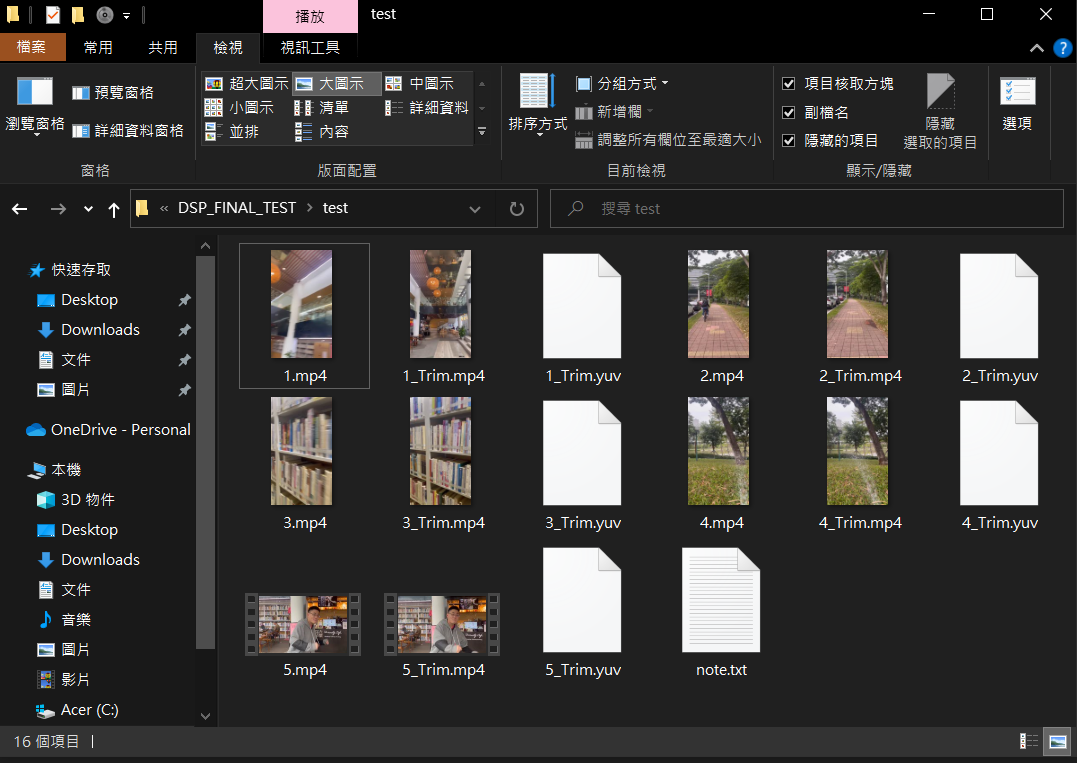
\includegraphics[width=0.80\textwidth]{0.png} 
\caption{测试资料表列结果}
\label{Test}
\end{figure}

\section{指令}

首先使用 FFMPEG 产生 YUV 档案,其产生过程的纪录如下。

1. 图书馆咖啡厅

\begin{lstlisting}[language={python}]
(base) PS D:\USERDATA\Desktop\DSP_FINAL_TEST\test> ffmpeg -i 1_Trim.mp4 -s 320x240 -pix_fmt yuv420p -r 15 1_Trim.yuv
ffmpeg version 2021-09-22-git-447cf53774-full_build-www.gyan.dev Copyright (c) 2000-2021 the FFmpeg developers
  built with gcc 10.3.0 (Rev5, Built by MSYS2 project)
  configuration: --enable-gpl --enable-version3 --enable-static --disable-w32threads --disable-autodetect --enable-fontconfig --enable-iconv --enable-gnutls --enable-libxml2 --enable-gmp --enable-lzma --enable-libsnappy --enable-zlib --enable-librist --enable-libsrt --enable-libssh --enable-libzmq --enable-avisynth --enable-libbluray --enable-libcaca --enable-sdl2 --enable-libdav1d --enable-libzvbi --enable-librav1e --enable-libsvtav1 --enable-libwebp --enable-libx264 --enable-libx265 --enable-libxvid --enable-libaom --enable-libopenjpeg --enable-libvpx --enable-libass --enable-frei0r --enable-libfreetype --enable-libfribidi --enable-libvidstab --enable-libvmaf --enable-libzimg --enable-amf --enable-cuda-llvm --enable-cuvid --enable-ffnvcodec --enable-nvdec --enable-nvenc --enable-d3d11va --enable-dxva2 --enable-libmfx --enable-libglslang --enable-vulkan --enable-opencl --enable-libcdio --enable-libgme --enable-libmodplug --enable-libopenmpt --enable-libopencore-amrwb --enable-libmp3lame --enable-libshine --enable-libtheora --enable-libtwolame --enable-libvo-amrwbenc --enable-libilbc --enable-libgsm --enable-libopencore-amrnb --enable-libopus --enable-libspeex --enable-libvorbis --enable-ladspa --enable-libbs2b --enable-libflite --enable-libmysofa --enable-librubberband --enable-libsoxr --enable-chromaprint
  libavutil      57.  6.100 / 57.  6.100
  libavcodec     59.  9.100 / 59.  9.100
  libavformat    59.  5.100 / 59.  5.100
  libavdevice    59.  0.101 / 59.  0.101
  libavfilter     8.  9.100 /  8.  9.100
  libswscale      6.  1.100 /  6.  1.100
  libswresample   4.  0.100 /  4.  0.100
  libpostproc    56.  0.100 / 56.  0.100
Input #0, mov,mp4,m4a,3gp,3g2,mj2, from '1_Trim.mp4':
  Metadata:
    major_brand     : mp42
    minor_version   : 0
    compatible_brands: mp41isom
    creation_time   : 2021-12-14T01:47:50.000000Z
  Duration: 00:00:04.19, start: 0.000000, bitrate: 3808 kb/s
  Stream #0:0[0x1](und): Video: h264 (Main) (avc1 / 0x31637661), yuv420p, 544x960 [SAR 1:1 DAR 17:30], 3700 kb/s, 30 fps, 30 tbr, 30k tbn (default)
    Metadata:
      creation_time   : 2021-12-18T06:23:36.000000Z
      handler_name    : VideoHandler
      vendor_id       : [0][0][0][0]
      encoder         : AVC Coding
  Stream #0:1[0x2](und): Audio: aac (LC) (mp4a / 0x6134706D), 48000 Hz, stereo, fltp, 180 kb/s (default)
    Metadata:
      creation_time   : 2021-12-18T06:23:36.000000Z
      handler_name    : SoundHandler
      vendor_id       : [0][0][0][0]
Stream mapping:
  Stream #0:0 -> #0:0 (h264 (native) -> rawvideo (native))
Press [q] to stop, [?] for help
Output #0, rawvideo, to '1_Trim.yuv':
  Metadata:
    major_brand     : mp42
    minor_version   : 0
    compatible_brands: mp41isom
    encoder         : Lavf59.5.100
  Stream #0:0(und): Video: rawvideo (I420 / 0x30323449), yuv420p(tv, progressive), 320x240 [SAR 17:40 DAR 17:30], q=2-31, 13824 kb/s, 15 fps, 15 tbn (default)
    Metadata:
      creation_time   : 2021-12-18T06:23:36.000000Z
      handler_name    : VideoHandler
      vendor_id       : [0][0][0][0]
      encoder         : Lavc59.9.100 rawvideo
frame=   63 fps=0.0 q=-0.0 Lsize=    7088kB time=00:00:04.20 bitrate=13824.0kbits/s dup=0 drop=60 speed=8.21x
video:7088kB audio:0kB subtitle:0kB other streams:0kB global headers:0kB muxing overhead: 0.000000%
(base) PS D:\USERDATA\Desktop\DSP_FINAL_TEST\test>
\end{lstlisting}

2. 图书馆旁的步道

\begin{lstlisting}[language={python}]
(base) PS D:\USERDATA\Desktop\DSP_FINAL_TEST\test> ffmpeg -i 2_Trim.mp4 -s 320x240 -pix_fmt yuv420p -r 15 2_Trim.yuv
ffmpeg version 2021-09-22-git-447cf53774-full_build-www.gyan.dev Copyright (c) 2000-2021 the FFmpeg developers
  built with gcc 10.3.0 (Rev5, Built by MSYS2 project)
  configuration: --enable-gpl --enable-version3 --enable-static --disable-w32threads --disable-autodetect --enable-fontconfig --enable-iconv --enable-gnutls --enable-libxml2 --enable-gmp --enable-lzma --enable-libsnappy --enable-zlib --enable-librist --enable-libsrt --enable-libssh --enable-libzmq --enable-avisynth --enable-libbluray --enable-libcaca --enable-sdl2 --enable-libdav1d --enable-libzvbi --enable-librav1e --enable-libsvtav1 --enable-libwebp --enable-libx264 --enable-libx265 --enable-libxvid --enable-libaom --enable-libopenjpeg --enable-libvpx --enable-libass --enable-frei0r --enable-libfreetype --enable-libfribidi --enable-libvidstab --enable-libvmaf --enable-libzimg --enable-amf --enable-cuda-llvm --enable-cuvid --enable-ffnvcodec --enable-nvdec --enable-nvenc --enable-d3d11va --enable-dxva2 --enable-libmfx --enable-libglslang --enable-vulkan --enable-opencl --enable-libcdio --enable-libgme --enable-libmodplug --enable-libopenmpt --enable-libopencore-amrwb --enable-libmp3lame --enable-libshine --enable-libtheora --enable-libtwolame --enable-libvo-amrwbenc --enable-libilbc --enable-libgsm --enable-libopencore-amrnb --enable-libopus --enable-libspeex --enable-libvorbis --enable-ladspa --enable-libbs2b --enable-libflite --enable-libmysofa --enable-librubberband --enable-libsoxr --enable-chromaprint
  libavutil      57.  6.100 / 57.  6.100
  libavcodec     59.  9.100 / 59.  9.100
  libavformat    59.  5.100 / 59.  5.100
  libavdevice    59.  0.101 / 59.  0.101
  libavfilter     8.  9.100 /  8.  9.100
  libswscale      6.  1.100 /  6.  1.100
  libswresample   4.  0.100 /  4.  0.100
  libpostproc    56.  0.100 / 56.  0.100
Input #0, mov,mp4,m4a,3gp,3g2,mj2, from '2_Trim.mp4':
  Metadata:
    major_brand     : mp42
    minor_version   : 0
    compatible_brands: mp41isom
    creation_time   : 2021-12-14T01:47:20.000000Z
  Duration: 00:00:04.98, start: 0.000000, bitrate: 11162 kb/s
  Stream #0:0[0x1](und): Video: h264 (Main) (avc1 / 0x31637661), yuv420p, 720x1280 [SAR 1:1 DAR 9:16], 11302 kb/s, 30 fps, 30 tbr, 30k tbn (default)
    Metadata:
      creation_time   : 2021-12-18T06:24:19.000000Z
      handler_name    : VideoHandler
      vendor_id       : [0][0][0][0]
      encoder         : AVC Coding
  Stream #0:1[0x2](und): Audio: aac (LC) (mp4a / 0x6134706D), 48000 Hz, stereo, fltp, 180 kb/s (default)
    Metadata:
      creation_time   : 2021-12-18T06:24:19.000000Z
      handler_name    : SoundHandler
      vendor_id       : [0][0][0][0]
Stream mapping:
  Stream #0:0 -> #0:0 (h264 (native) -> rawvideo (native))
Press [q] to stop, [?] for help
Output #0, rawvideo, to '2_Trim.yuv':
  Metadata:
    major_brand     : mp42
    minor_version   : 0
    compatible_brands: mp41isom
    encoder         : Lavf59.5.100
  Stream #0:0(und): Video: rawvideo (I420 / 0x30323449), yuv420p(tv, progressive), 320x240 [SAR 27:64 DAR 9:16], q=2-31, 13824 kb/s, 15 fps, 15 tbn (default)
    Metadata:
      creation_time   : 2021-12-18T06:24:19.000000Z
      handler_name    : VideoHandler
      vendor_id       : [0][0][0][0]
      encoder         : Lavc59.9.100 rawvideo
frame=   75 fps=0.0 q=-0.0 Lsize=    8438kB time=00:00:05.00 bitrate=13824.0kbits/s dup=1 drop=71 speed= 5.6x
video:8438kB audio:0kB subtitle:0kB other streams:0kB global headers:0kB muxing overhead: 0.000000%
(base) PS D:\USERDATA\Desktop\DSP_FINAL_TEST\test>
\end{lstlisting}

3. 图书馆内书架陈列

\begin{lstlisting}[language={python}]
(base) PS D:\USERDATA\Desktop\DSP_FINAL_TEST\test> ffmpeg -i 3_Trim.mp4 -s 320x240 -pix_fmt yuv420p -r 15 3_Trim.yuv
ffmpeg version 2021-09-22-git-447cf53774-full_build-www.gyan.dev Copyright (c) 2000-2021 the FFmpeg developers
  built with gcc 10.3.0 (Rev5, Built by MSYS2 project)
  configuration: --enable-gpl --enable-version3 --enable-static --disable-w32threads --disable-autodetect --enable-fontconfig --enable-iconv --enable-gnutls --enable-libxml2 --enable-gmp --enable-lzma --enable-libsnappy --enable-zlib --enable-librist --enable-libsrt --enable-libssh --enable-libzmq --enable-avisynth --enable-libbluray --enable-libcaca --enable-sdl2 --enable-libdav1d --enable-libzvbi --enable-librav1e --enable-libsvtav1 --enable-libwebp --enable-libx264 --enable-libx265 --enable-libxvid --enable-libaom --enable-libopenjpeg --enable-libvpx --enable-libass --enable-frei0r --enable-libfreetype --enable-libfribidi --enable-libvidstab --enable-libvmaf --enable-libzimg --enable-amf --enable-cuda-llvm --enable-cuvid --enable-ffnvcodec --enable-nvdec --enable-nvenc --enable-d3d11va --enable-dxva2 --enable-libmfx --enable-libglslang --enable-vulkan --enable-opencl --enable-libcdio --enable-libgme --enable-libmodplug --enable-libopenmpt --enable-libopencore-amrwb --enable-libmp3lame --enable-libshine --enable-libtheora --enable-libtwolame --enable-libvo-amrwbenc --enable-libilbc --enable-libgsm --enable-libopencore-amrnb --enable-libopus --enable-libspeex --enable-libvorbis --enable-ladspa --enable-libbs2b --enable-libflite --enable-libmysofa --enable-librubberband --enable-libsoxr --enable-chromaprint
  libavutil      57.  6.100 / 57.  6.100
  libavcodec     59.  9.100 / 59.  9.100
  libavformat    59.  5.100 / 59.  5.100
  libavdevice    59.  0.101 / 59.  0.101
  libavfilter     8.  9.100 /  8.  9.100
  libswscale      6.  1.100 /  6.  1.100
  libswresample   4.  0.100 /  4.  0.100
  libpostproc    56.  0.100 / 56.  0.100
Input #0, mov,mp4,m4a,3gp,3g2,mj2, from '3_Trim.mp4':
  Metadata:
    major_brand     : mp42
    minor_version   : 0
    compatible_brands: mp41isom
    creation_time   : 2021-12-14T01:47:41.000000Z
  Duration: 00:00:04.89, start: 0.000000, bitrate: 3705 kb/s
  Stream #0:0[0x1](und): Video: h264 (Main) (avc1 / 0x31637661), yuv420p, 544x960 [SAR 1:1 DAR 17:30], 3643 kb/s, 30 fps, 30 tbr, 30k tbn (default)
    Metadata:
      creation_time   : 2021-12-18T06:24:54.000000Z
      handler_name    : VideoHandler
      vendor_id       : [0][0][0][0]
      encoder         : AVC Coding
  Stream #0:1[0x2](und): Audio: aac (LC) (mp4a / 0x6134706D), 48000 Hz, stereo, fltp, 176 kb/s (default)
    Metadata:
      creation_time   : 2021-12-18T06:24:54.000000Z
      handler_name    : SoundHandler
      vendor_id       : [0][0][0][0]
Stream mapping:
  Stream #0:0 -> #0:0 (h264 (native) -> rawvideo (native))
Press [q] to stop, [?] for help
Output #0, rawvideo, to '3_Trim.yuv':
  Metadata:
    major_brand     : mp42
    minor_version   : 0
    compatible_brands: mp41isom
    encoder         : Lavf59.5.100
  Stream #0:0(und): Video: rawvideo (I420 / 0x30323449), yuv420p(tv, progressive), 320x240 [SAR 17:40 DAR 17:30], q=2-31, 13824 kb/s, 15 fps, 15 tbn (default)
    Metadata:
      creation_time   : 2021-12-18T06:24:54.000000Z
      handler_name    : VideoHandler
      vendor_id       : [0][0][0][0]
      encoder         : Lavc59.9.100 rawvideo
frame=   74 fps=0.0 q=-0.0 Lsize=    8325kB time=00:00:04.93 bitrate=13824.0kbits/s dup=1 drop=69 speed=12.2x
video:8325kB audio:0kB subtitle:0kB other streams:0kB global headers:0kB muxing overhead: 0.000000%
(base) PS D:\USERDATA\Desktop\DSP_FINAL_TEST\test>
\end{lstlisting}

4. 图书馆旁的草皮

\begin{lstlisting}[language={python}]
(base) PS D:\USERDATA\Desktop\DSP_FINAL_TEST\test> ffmpeg -i 4_Trim.mp4 -s 320x240 -pix_fmt yuv420p -r 15 4_Trim.yuv
ffmpeg version 2021-09-22-git-447cf53774-full_build-www.gyan.dev Copyright (c) 2000-2021 the FFmpeg developers
  built with gcc 10.3.0 (Rev5, Built by MSYS2 project)
  configuration: --enable-gpl --enable-version3 --enable-static --disable-w32threads --disable-autodetect --enable-fontconfig --enable-iconv --enable-gnutls --enable-libxml2 --enable-gmp --enable-lzma --enable-libsnappy --enable-zlib --enable-librist --enable-libsrt --enable-libssh --enable-libzmq --enable-avisynth --enable-libbluray --enable-libcaca --enable-sdl2 --enable-libdav1d --enable-libzvbi --enable-librav1e --enable-libsvtav1 --enable-libwebp --enable-libx264 --enable-libx265 --enable-libxvid --enable-libaom --enable-libopenjpeg --enable-libvpx --enable-libass --enable-frei0r --enable-libfreetype --enable-libfribidi --enable-libvidstab --enable-libvmaf --enable-libzimg --enable-amf --enable-cuda-llvm --enable-cuvid --enable-ffnvcodec --enable-nvdec --enable-nvenc --enable-d3d11va --enable-dxva2 --enable-libmfx --enable-libglslang --enable-vulkan --enable-opencl --enable-libcdio --enable-libgme --enable-libmodplug --enable-libopenmpt --enable-libopencore-amrwb --enable-libmp3lame --enable-libshine --enable-libtheora --enable-libtwolame --enable-libvo-amrwbenc --enable-libilbc --enable-libgsm --enable-libopencore-amrnb --enable-libopus --enable-libspeex --enable-libvorbis --enable-ladspa --enable-libbs2b --enable-libflite --enable-libmysofa --enable-librubberband --enable-libsoxr --enable-chromaprint
  libavutil      57.  6.100 / 57.  6.100
  libavcodec     59.  9.100 / 59.  9.100
  libavformat    59.  5.100 / 59.  5.100
  libavdevice    59.  0.101 / 59.  0.101
  libavfilter     8.  9.100 /  8.  9.100
  libswscale      6.  1.100 /  6.  1.100
  libswresample   4.  0.100 /  4.  0.100
  libpostproc    56.  0.100 / 56.  0.100
Input #0, mov,mp4,m4a,3gp,3g2,mj2, from '4_Trim.mp4':
  Metadata:
    major_brand     : mp42
    minor_version   : 0
    compatible_brands: mp41isom
    creation_time   : 2021-12-14T01:47:31.000000Z
  Duration: 00:00:04.87, start: 0.000000, bitrate: 14394 kb/s
  Stream #0:0[0x1](und): Video: h264 (Main) (avc1 / 0x31637661), yuv420p, 720x1280 [SAR 1:1 DAR 9:16], 14600 kb/s, 30 fps, 30 tbr, 30k tbn (default)
    Metadata:
      creation_time   : 2021-12-18T06:26:14.000000Z
      handler_name    : VideoHandler
      vendor_id       : [0][0][0][0]
      encoder         : AVC Coding
  Stream #0:1[0x2](und): Audio: aac (LC) (mp4a / 0x6134706D), 48000 Hz, stereo, fltp, 198 kb/s (default)
    Metadata:
      creation_time   : 2021-12-18T06:26:14.000000Z
      handler_name    : SoundHandler
      vendor_id       : [0][0][0][0]
Stream mapping:
  Stream #0:0 -> #0:0 (h264 (native) -> rawvideo (native))
Press [q] to stop, [?] for help
Output #0, rawvideo, to '4_Trim.yuv':
  Metadata:
    major_brand     : mp42
    minor_version   : 0
    compatible_brands: mp41isom
    encoder         : Lavf59.5.100
  Stream #0:0(und): Video: rawvideo (I420 / 0x30323449), yuv420p(tv, progressive), 320x240 [SAR 27:64 DAR 9:16], q=2-31, 13824 kb/s, 15 fps, 15 tbn (default)
    Metadata:
      creation_time   : 2021-12-18T06:26:14.000000Z
      handler_name    : VideoHandler
      vendor_id       : [0][0][0][0]
      encoder         : Lavc59.9.100 rawvideo
frame=   74 fps=0.0 q=-0.0 Lsize=    8325kB time=00:00:04.93 bitrate=13824.0kbits/s dup=1 drop=69 speed=5.28x
video:8325kB audio:0kB subtitle:0kB other streams:0kB global headers:0kB muxing overhead: 0.000000%
(base) PS D:\USERDATA\Desktop\DSP_FINAL_TEST\test>
\end{lstlisting}

5. 隐藏人物

\begin{lstlisting}[language={python}]
(base) PS D:\USERDATA\Desktop\DSP_FINAL_TEST\test> ffmpeg -i 5_Trim.mp4 -s 320x240 -pix_fmt yuv420p -r 15 5_Trim.yuv
ffmpeg version 2021-09-22-git-447cf53774-full_build-www.gyan.dev Copyright (c) 2000-2021 the FFmpeg developers
  built with gcc 10.3.0 (Rev5, Built by MSYS2 project)
  configuration: --enable-gpl --enable-version3 --enable-static --disable-w32threads --disable-autodetect --enable-fontconfig --enable-iconv --enable-gnutls --enable-libxml2 --enable-gmp --enable-lzma --enable-libsnappy --enable-zlib --enable-librist --enable-libsrt --enable-libssh --enable-libzmq --enable-avisynth --enable-libbluray --enable-libcaca --enable-sdl2 --enable-libdav1d --enable-libzvbi --enable-librav1e --enable-libsvtav1 --enable-libwebp --enable-libx264 --enable-libx265 --enable-libxvid --enable-libaom --enable-libopenjpeg --enable-libvpx --enable-libass --enable-frei0r --enable-libfreetype --enable-libfribidi --enable-libvidstab --enable-libvmaf --enable-libzimg --enable-amf --enable-cuda-llvm --enable-cuvid --enable-ffnvcodec --enable-nvdec --enable-nvenc --enable-d3d11va --enable-dxva2 --enable-libmfx --enable-libglslang --enable-vulkan --enable-opencl --enable-libcdio --enable-libgme --enable-libmodplug --enable-libopenmpt --enable-libopencore-amrwb --enable-libmp3lame --enable-libshine --enable-libtheora --enable-libtwolame --enable-libvo-amrwbenc --enable-libilbc --enable-libgsm --enable-libopencore-amrnb --enable-libopus --enable-libspeex --enable-libvorbis --enable-ladspa --enable-libbs2b --enable-libflite --enable-libmysofa --enable-librubberband --enable-libsoxr --enable-chromaprint
  libavutil      57.  6.100 / 57.  6.100
  libavcodec     59.  9.100 / 59.  9.100
  libavformat    59.  5.100 / 59.  5.100
  libavdevice    59.  0.101 / 59.  0.101
  libavfilter     8.  9.100 /  8.  9.100
  libswscale      6.  1.100 /  6.  1.100
  libswresample   4.  0.100 /  4.  0.100
  libpostproc    56.  0.100 / 56.  0.100
Input #0, mov,mp4,m4a,3gp,3g2,mj2, from '5_Trim.mp4':
  Metadata:
    major_brand     : mp42
    minor_version   : 0
    compatible_brands: mp41isom
    creation_time   : 2021-12-14T01:47:59.000000Z
  Duration: 00:00:04.93, start: 0.000000, bitrate: 4755 kb/s
  Stream #0:0[0x1](und): Video: h264 (Main) (avc1 / 0x31637661), yuv420p, 1280x720 [SAR 1:1 DAR 16:9], 4733 kb/s, 30 fps, 30 tbr, 30k tbn (default)
    Metadata:
      creation_time   : 2021-12-18T06:27:01.000000Z
      handler_name    : VideoHandler
      vendor_id       : [0][0][0][0]
      encoder         : AVC Coding
  Stream #0:1[0x2](und): Audio: aac (LC) (mp4a / 0x6134706D), 48000 Hz, stereo, fltp, 179 kb/s (default)
    Metadata:
      creation_time   : 2021-12-18T06:27:01.000000Z
      handler_name    : SoundHandler
      vendor_id       : [0][0][0][0]
Stream mapping:
  Stream #0:0 -> #0:0 (h264 (native) -> rawvideo (native))
Press [q] to stop, [?] for help
Output #0, rawvideo, to '5_Trim.yuv':
  Metadata:
    major_brand     : mp42
    minor_version   : 0
    compatible_brands: mp41isom
    encoder         : Lavf59.5.100
  Stream #0:0(und): Video: rawvideo (I420 / 0x30323449), yuv420p(tv, progressive), 320x240 [SAR 4:3 DAR 16:9], q=2-31, 13824 kb/s, 15 fps, 15 tbn (default)
    Metadata:
      creation_time   : 2021-12-18T06:27:01.000000Z
      handler_name    : VideoHandler
      vendor_id       : [0][0][0][0]
      encoder         : Lavc59.9.100 rawvideo
frame=   74 fps=0.0 q=-0.0 Lsize=    8325kB time=00:00:04.93 bitrate=13824.0kbits/s dup=1 drop=70 speed=8.97x
video:8325kB audio:0kB subtitle:0kB other streams:0kB global headers:0kB muxing overhead: 0.000000%
(base) PS D:\USERDATA\Desktop\DSP_FINAL_TEST\test>
\end{lstlisting}

各指令记录如下 :

\begin{lstlisting}[language={python}]
ffmpeg -i 1_Trim.mp4 -s 320x240 -pix_fmt yuv420p -r 15 1_Trim.yuv

ffmpeg -i 2_Trim.mp4 -s 320x240 -pix_fmt yuv420p -r 15 2_Trim.yuv

ffmpeg -i 3_Trim.mp4 -s 320x240 -pix_fmt yuv420p -r 15 3_Trim.yuv

ffmpeg -i 4_Trim.mp4 -s 320x240 -pix_fmt yuv420p -r 15 4_Trim.yuv

ffmpeg -i 5_Trim.mp4 -s 320x240 -pix_fmt yuv420p -r 15 5_Trim.yuv

ffplay -video_size 320x240 -i 1_Trim.yuv

ffplay -video_size 320x240 -i 2_Trim.yuv

ffplay -video_size 320x240 -i 3_Trim.yuv

ffplay -video_size 320x240 -i 4_Trim.yuv

ffplay -video_size 320x240 -i 5_Trim.yuv
\end{lstlisting}

最后播放结果如下 :

\begin{figure}[H]
\centering 
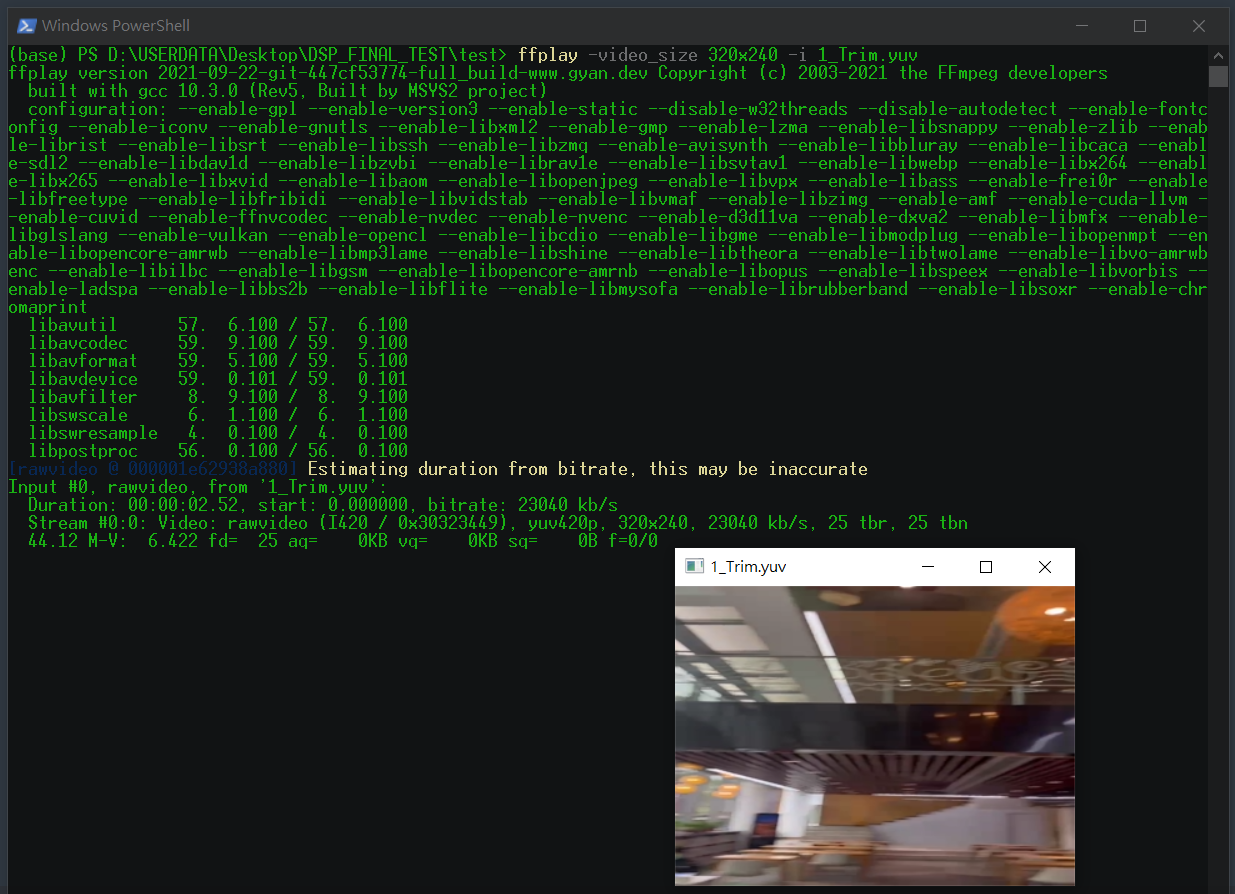
\includegraphics[width=0.80\textwidth]{1.png} 
\caption{图书馆咖啡厅}
\label{Test}
\end{figure}

\begin{figure}[H]
\centering 
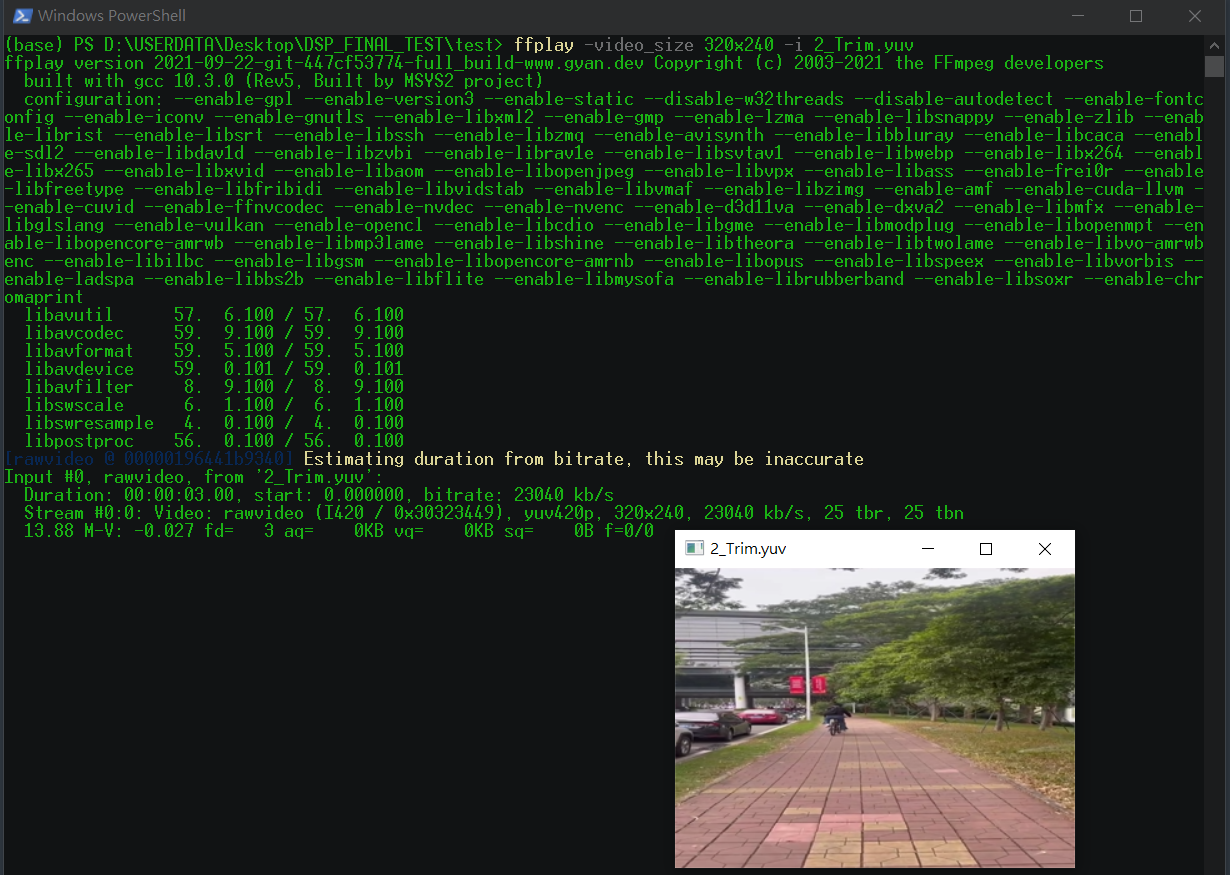
\includegraphics[width=0.80\textwidth]{2.png} 
\caption{图书馆旁的步道}
\label{Test}
\end{figure}

\begin{figure}[H]
\centering 
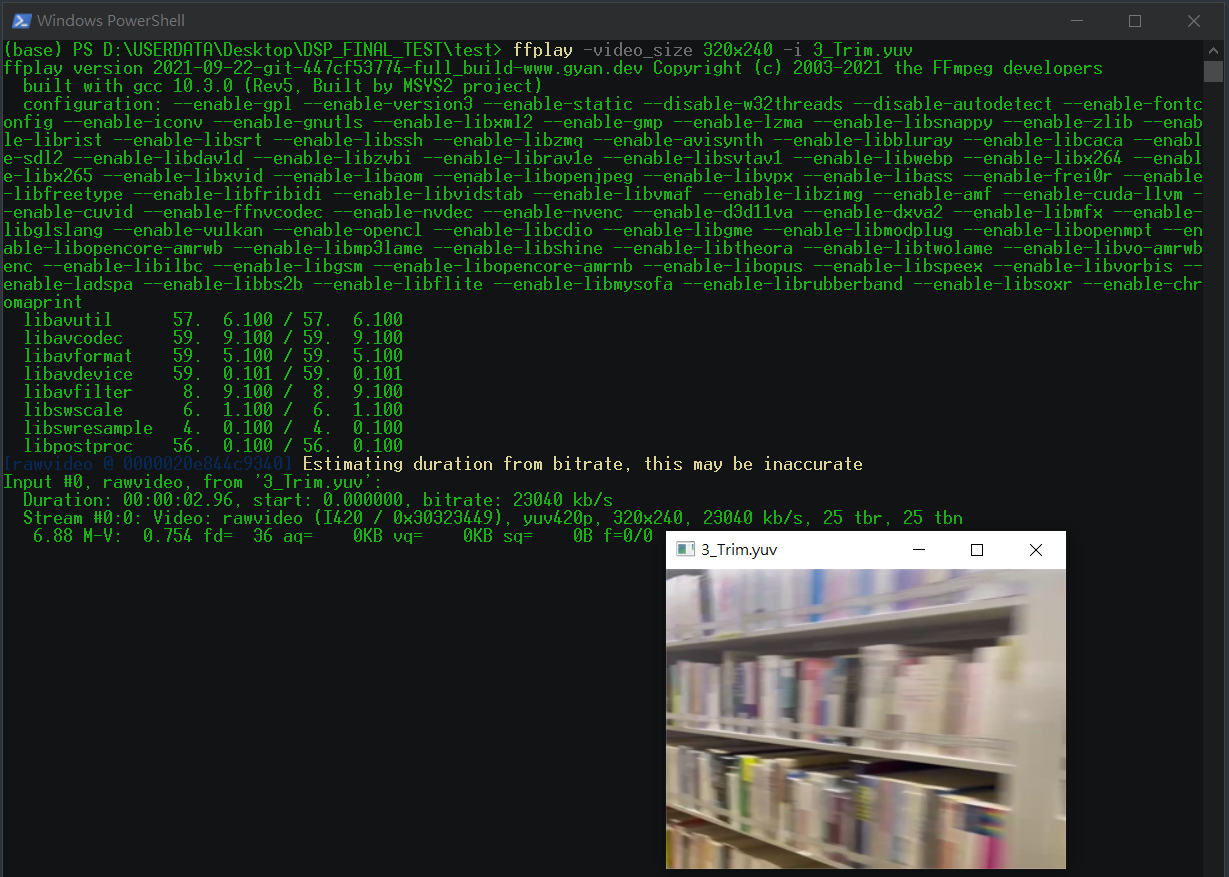
\includegraphics[width=0.80\textwidth]{3.png} 
\caption{图书馆内书架陈列}
\label{Test}
\end{figure}

\begin{figure}[H]
\centering 
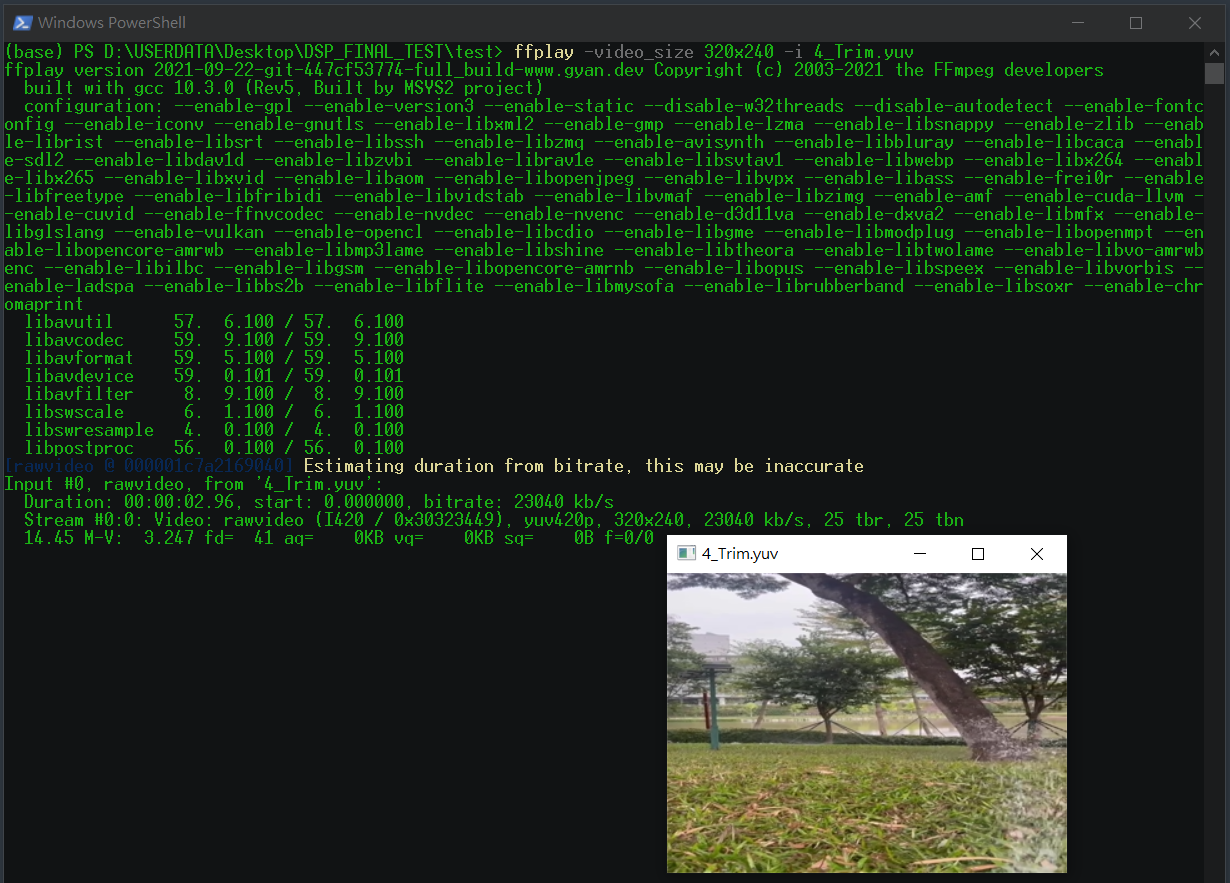
\includegraphics[width=0.80\textwidth]{4.png} 
\caption{图书馆旁的草皮}
\label{Test}
\end{figure}

\begin{figure}[H]
\centering 
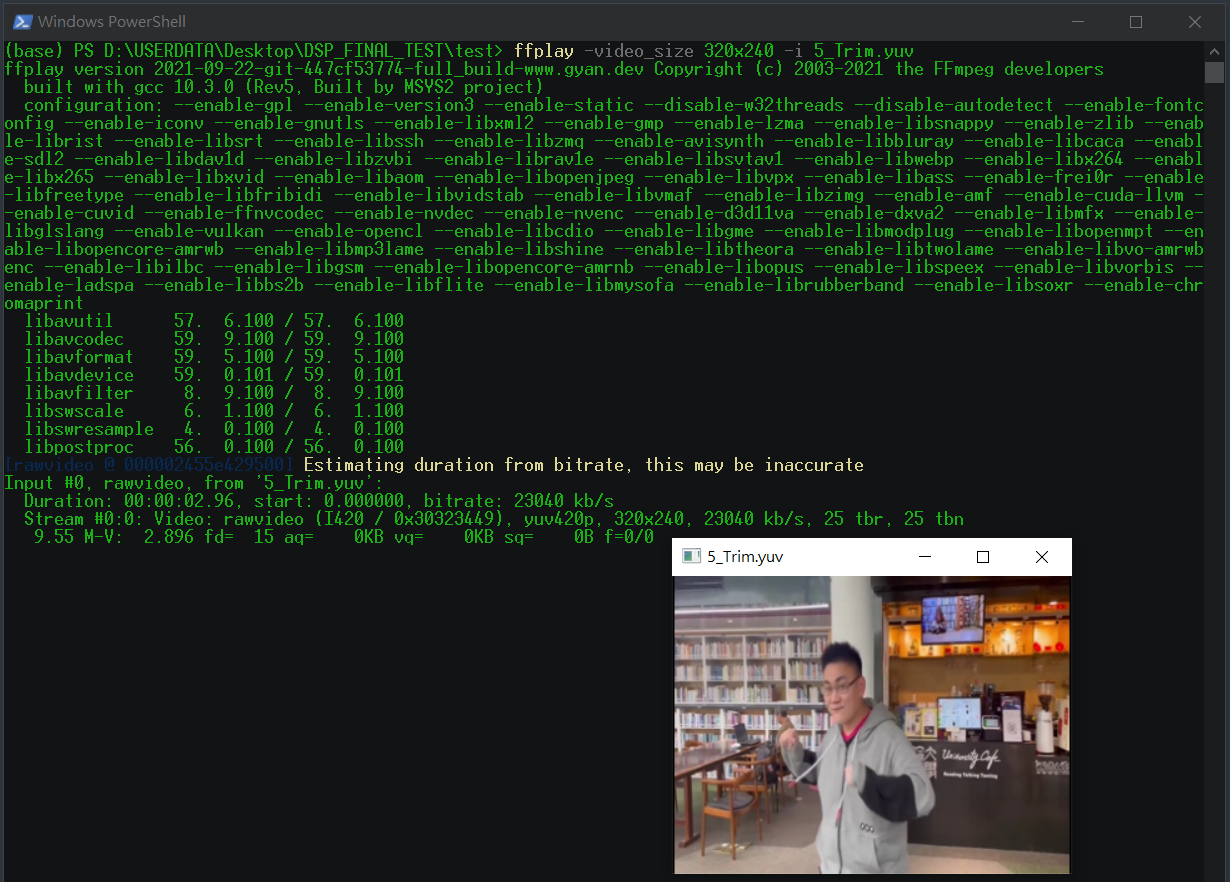
\includegraphics[width=0.80\textwidth]{5.png} 
\caption{隐藏人物}
\label{Test}
\end{figure}

\newpage

\section{结果}

从实验结果可知,从 10 到 9 的阶段就有很大的效果呈现,而后续有反弹的微幅增加,但随后又下降。。



\begin{figure}[H]
\centering 
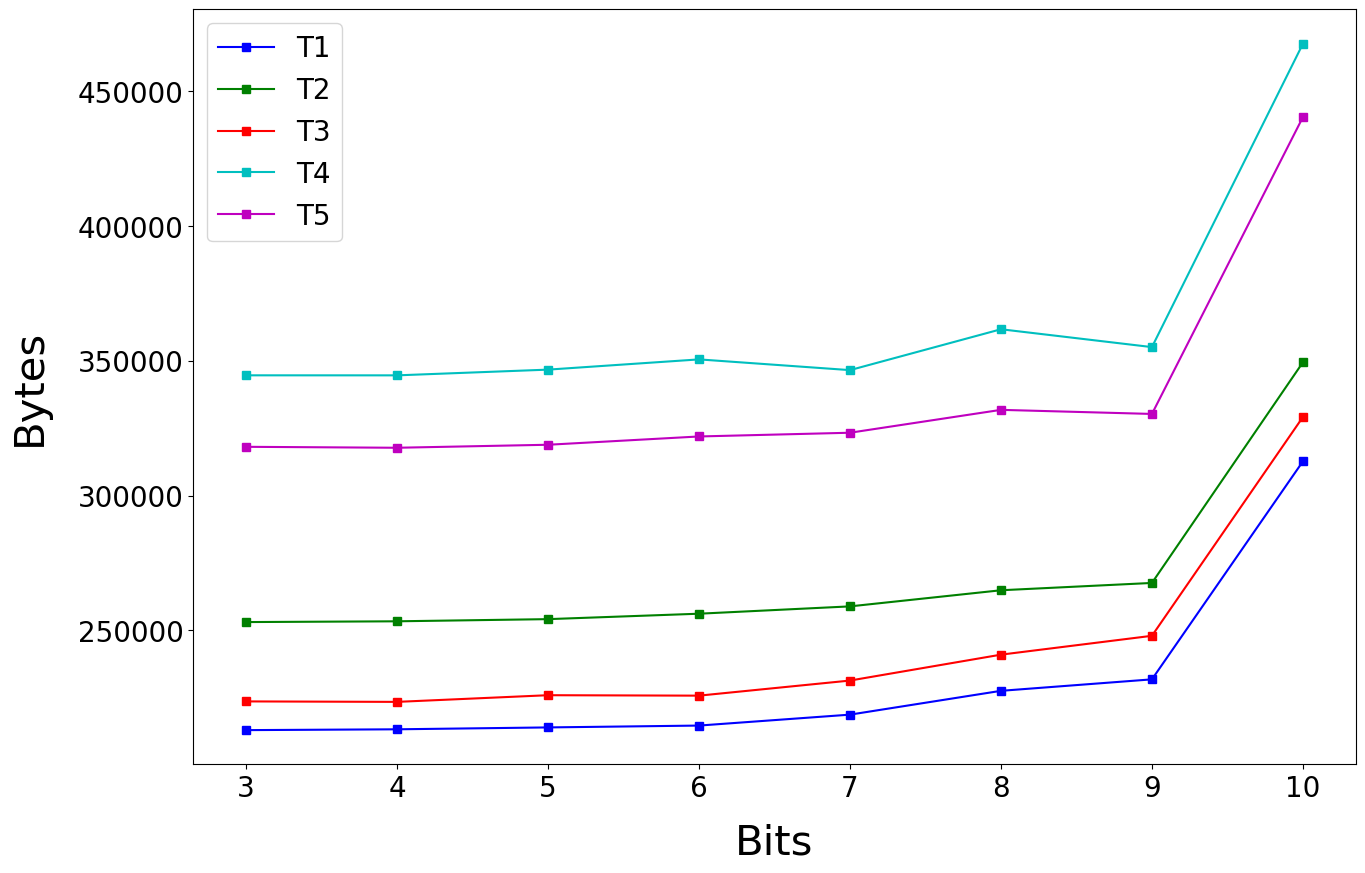
\includegraphics[width=0.80\textwidth]{r1.png} 
\caption{测试结果}
\label{Test}
\end{figure}

\begin{figure}[H]
\centering 
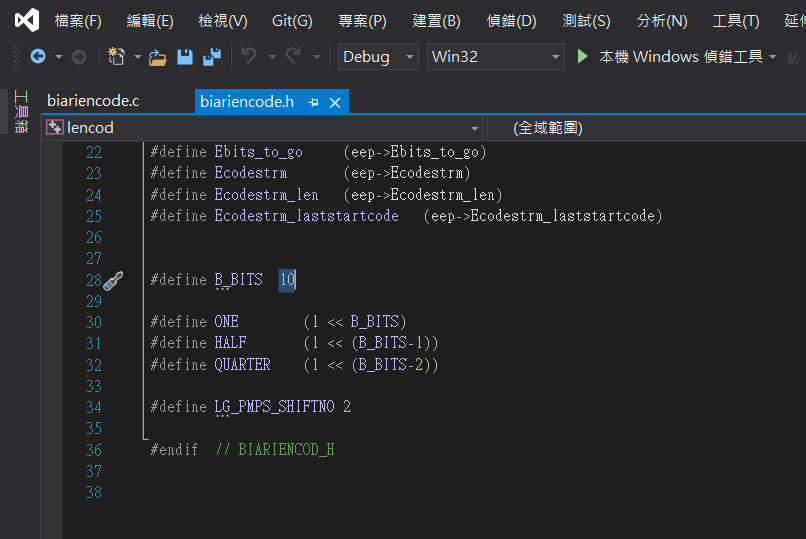
\includegraphics[width=0.80\textwidth]{r2.png} 
\caption{改动示意}
\label{Test}
\end{figure}

\begin{figure}[H]
\centering 
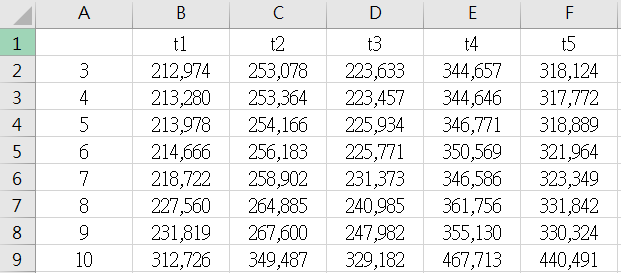
\includegraphics[width=0.80\textwidth]{r3.png} 
\caption{数据呈现}
\label{Test}
\end{figure}

%\section{附錄}

% 數學意義說明

% $$\min \limits_{G}\max \limits_{D}{V_I(D,\ G)=V(D,G)-\lambda L_I(G,Q)}$$

%	\begin{lstlisting}[language={python}]

%	\end{lstlisting}

%\begin{enumerate}
%\item Y
%\item A
%\end{enumerate}

% \newpage

\clearpage

\end{document}